%//////////////////////////////////
%/// P R E A M B L E

\documentclass[a4paper, 12pt]{article}

\usepackage[utf8]{inputenc}
\usepackage[singlespacing]{setspace}
\usepackage{amsmath}
\usepackage{mathtools}
\usepackage{caption}
\usepackage{float}
\usepackage{booktabs}
\usepackage{graphicx}
\usepackage{multicol}
\usepackage{gensymb}
\usepackage{breqn}
\usepackage{indentfirst}
\usepackage{siunitx}
\usepackage{tabularx, booktabs}
\newcolumntype{Y}{>{\centering\arraybackslash}X}

\usepackage{pdfpages}

\usepackage{multicol}
\usepackage{supertabular}

\usepackage{svg}

\widowpenalty = 4500
\clubpenalty  = 4500

\setlength{\jot}{10pt} %indents


\newcommand*\dif{\mathop{}\!\mathrm{d}}
\newcommand*\shortminus{\scalebox{0.5}[1.0]{\( - \)}}
%\newcommand{\euler}{\mathrm{e}}
%\newcommand{\ramuno}{\mathrm{j}}

%%========================================
%% circuitikz properties
\usepackage[european, straightvoltages]{circuitikz}
%\ctikzvalof{voltage/distance from node = .2}
%\ctikzset{voltage/distance from node  =.5}% in \pgf@circ@Rlen units
%\ctikzset{voltage/distance from line  =.25}% pos. between 0 and 1
%\ctikzset{voltage/bump b/.initial     =1.5}%

\ctikzset{current/distance            = .618}


%%========================================

%%
%% Path settings
%%
\graphicspath{ {./graphics/} }


%//////////////////////////////////
%/// D O C U M E N T
\begin{document}

%%%%%%%%%%%%%%%%%%%%%%%%%%%%%%%%%%%%%
  %\includepdf{Deckblatt.pdf}
  
\includepdf{./titlepage/titlepage.pdf}
%%%%%%%%%%%%%%%%%%%%%%%%%%%%%%%%%%%%%

\section{Vorbereitungsaufgaben}

  % 2.1
  \subsection{}
    \begin{center}
      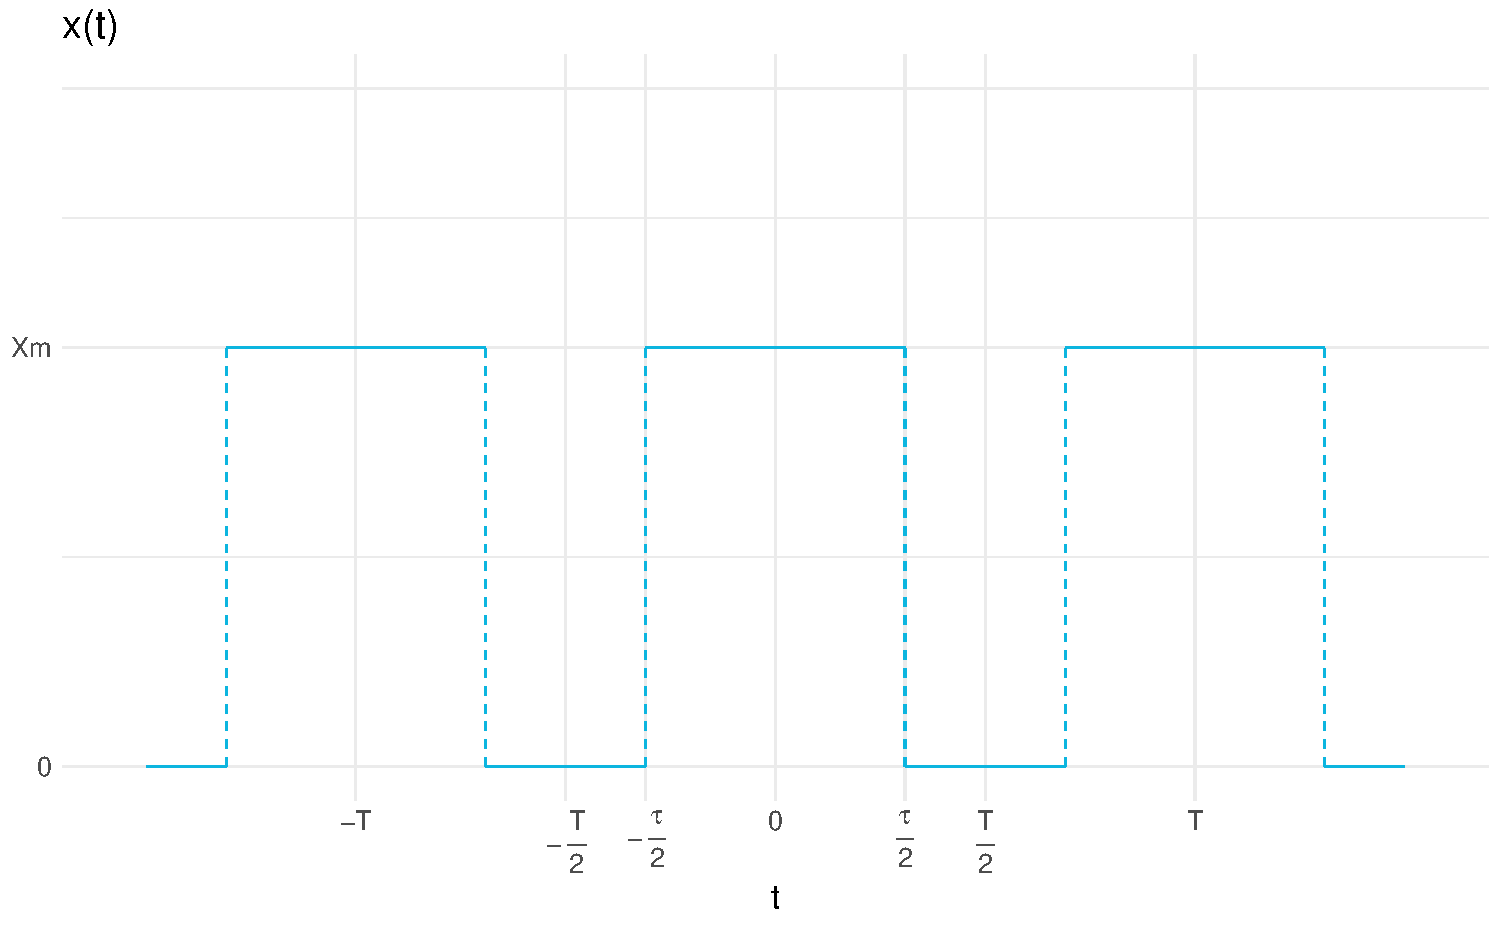
\includegraphics[scale=0.5]{./R/2_1/2_1_function.pdf}
    \end{center}

    \begin{align*}
      \underline{X}_\nu &= \frac{1}{T_1} \cdot \int_{T_1}{x(t) \cdot e^{-(j\nu\cdot\omega_1t)}\dif t}\\
      &= \frac{1}{T_1} \cdot \int_{\shortminus\frac{\tau}{2}}^{\frac{\tau}{2}}{ X_m \cdot e^{-(j\nu\cdot\omega_1t)}\dif t}\\
      &= - \frac{X_m}{T_1 \cdot j \nu \omega_1 } \cdot \left[  e^{-(j\nu\cdot\omega_1t)} \right]^{\frac{\tau}{2}}_{\shortminus\frac{\tau}{2}}\\
      &= -\frac{X_m}{T_1 \cdot j \nu \omega_1 } \cdot \left ( e^{-j\nu\cdot\omega_1 \frac{\tau}{2}} - e^{j\nu\cdot\omega_1 \frac{\tau}{2}} \right )
      %
      \intertext{$\omega_1 = \frac{2 \pi}{T_1}$ und Erweiterung mit $\frac{-1}{-1}$:}
      \underline{X}_\nu &= \frac{X_m}{2 j \pi \nu } \cdot \left ( e^{j\nu\cdot \pi \frac{\tau}{T_1}} - e^{-j\nu\cdot \pi \frac{\tau}{T_1}} \right )\\
      &= \frac{X_m}{\pi \nu } \cdot \frac{\left ( e^{j\nu\cdot \pi \frac{\tau}{T_1}} - e^{-j\nu\cdot \pi \frac{\tau}{T_1}} \right )}{2 j}
    \end{align*}

    \begin{gather*}
      \text{\small{ mit $ \frac{\left ( e^{jx} - e^{-jx} \right )}{2 j} = \sin{(x)}$ und $\frac{\tau}{T_1} = D$: }}\notag\\
      \underline{X}_\nu = \frac{X_m}{\pi \nu } \cdot \sin{(\pi \nu D)}
    \end{gather*}

    \begin{gather*}
        \text{\small Erweitert man wieder mit $\frac{D}{D}$ erhält man das Bild einer Spaltfunktion $\text{si}(x)=\frac{\sin x }{x}$: }\notag\\
        \underline{X}_\nu = D \cdot X_m \cdot \frac{\sin(\pi \nu D)}{\pi \nu D} = D \cdot X_m \cdot \text{si}(\pi \nu D)
      %\shortintertext{or}
    \end{gather*}

    \begin{gather*}
        \text{\small Als reele Reihe:}\notag\\
        x(t) = X_0 + \sum^{\infty}_{\nu=1}{\hat{X}_\nu \cos(\nu \cdot \omega_1 t + \phi_\nu )}\\
        X_0 = \frac{1}{T_1} \cdot \int_{T_1}{x(t) \dif t} = \frac{X_m}{2}\\
    \end{gather*}

    \begin{gather*}
      \text{\small Aus der komplexen Reihendarstellung folgt}\notag\\
      \hat{X}_\nu = \sqrt{a^2_\nu + b^2_\nu}\\
      \phi_\nu = \arccos{\frac{a_\nu}{\hat{X}_\nu}}\\
      a_\nu = 2 \cdot \text{Re}(\underline{X}_\nu) = 2 D X_m \cdot \text{si}(\pi \nu D)\\
      b_\nu = -2 \cdot \text{Im}(\underline{X}_\nu) = 0\\
      \text{\small also}\notag\\
      a_\nu = \hat{X}_\nu, \,\
      \phi_\nu = 0
    \end{gather*}

    \begin{gather*}
      \text{\small Somit ist}\notag\\
      x(t) = \frac{X_m}{2} + \sum^{\infty}_{\nu=1}{2 D X_m \cdot \text{si}(\pi \nu D) \cdot \cos(\nu \cdot \frac{2\pi}{T_1} \cdot t)}
    \end{gather*}

    \vspace{0.021276873\paperheight}

    \begin{center}
      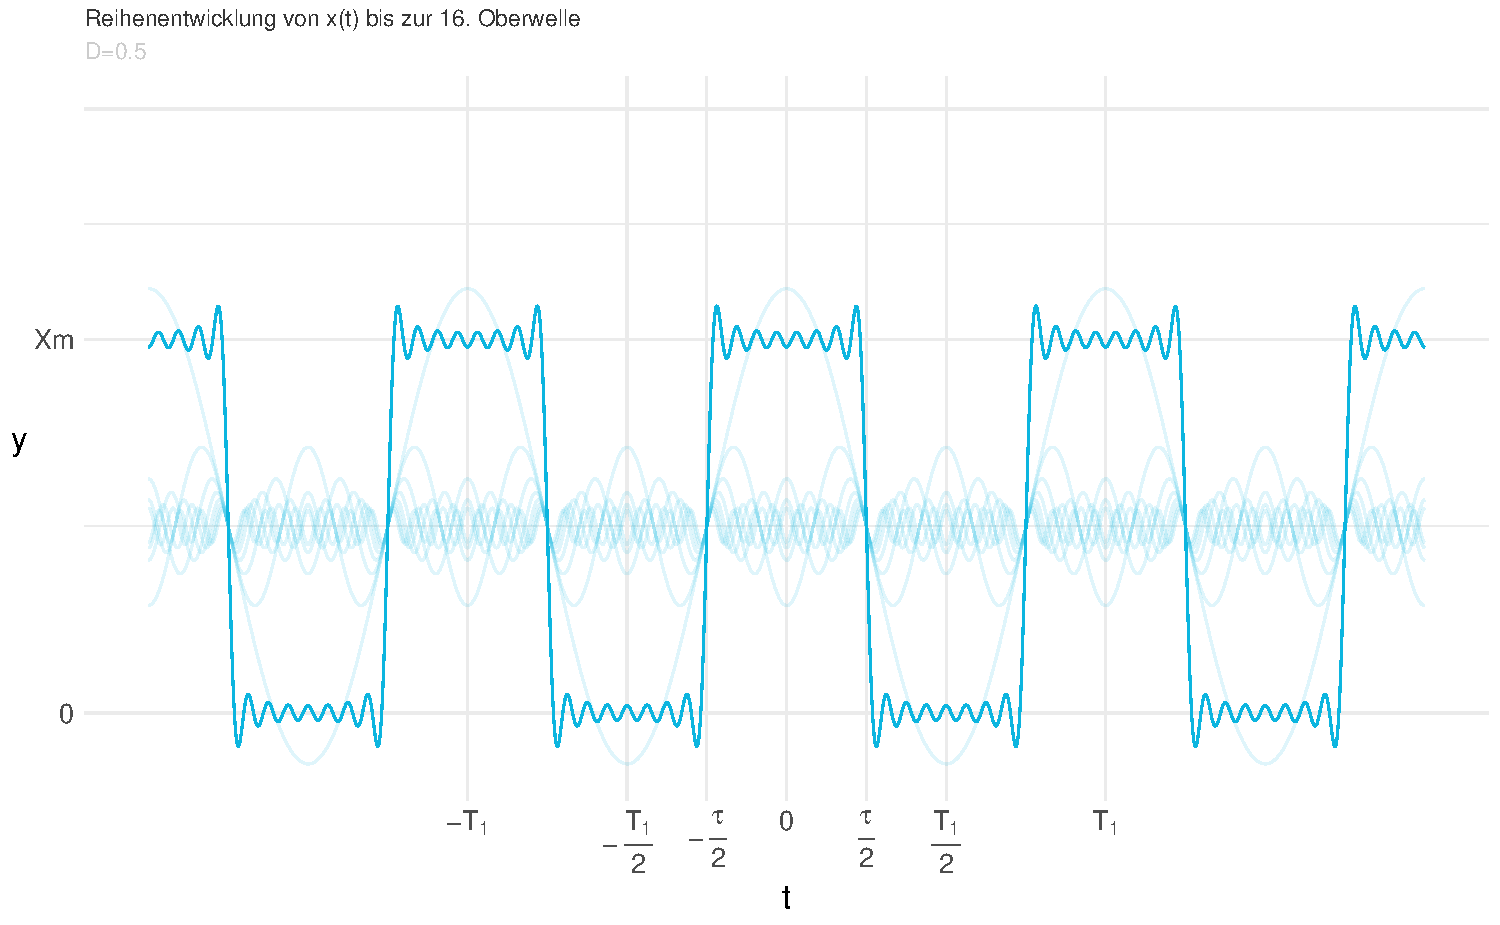
\includegraphics[scale=0.5]{./R/2_1/2_1_Reihe.pdf}
    \end{center}

    \begin{gather*}
      \text{\small Effektivwert:}\notag\\
      X_{\text{eff}} = \sqrt{ \frac{1}{T_1} \cdot \int_{T_1}{x^2(t) \dif t} } = \sqrt{ \frac{X_m^2}{T_1} \cdot \int_{\shortminus\frac{\tau}{2}}^{\frac{\tau}{2}}{1 \dif t} }\\
      X_{\text{eff}}= X_m \cdot \sqrt{\frac{\tau}{T_1}} = X_m \cdot \sqrt{D}
    \end{gather*}

    %\vspace{0.021276873\paperheight}
    \begin{table}[H]
      \begin{center}
        \begin{tabular}{@{}cccc@{}}
        \toprule
        \multicolumn{3}{c}{$D = \frac{1}{2}$} \\ \midrule
        $\nu$      & $\hat{X}_\nu$   & $\phi_\nu$ & $X_{\text{eff}}$   \\ \hline
        0          &  $$         &       &       \\
        1          &  $$         &        &      \\
        2          &  $$     &            &      \\
        3          &  $$        &         &     \\
        4          &  $$         &        &      \\
        5          &  $$        &         &     \\
        6          &  $$        &          &    \\
        7          &  $$         &         &     \\
        8          &  $$         &         &     \\
        9          &  $$         &         &     \\
        10         &  $$         &         &     \\
        13         &  $$         &         &     \\
        14         &  $$         &         &     \\
        15         &  $$         &         &     \\
        16         &  $$         &         &     \\ \bottomrule
        \end{tabular}
      \end{center}
    \end{table}

    \begin{gather*}
    \end{gather*}

  % 2.2
  \subsection{}

  % 2.3
  \subsection{}

\section{Versuchsaufgaben}
  % 3.1
  \subsection{}

  % 3.2
  \subsection{}
  
  % 3.3
  \subsection{}


\end{document}
